\documentclass[a4paper, 9pt]{scrartcl}\usepackage[]{graphicx}\usepackage[]{xcolor}
% maxwidth is the original width if it is less than linewidth
% otherwise use linewidth (to make sure the graphics do not exceed the margin)
\makeatletter
\def\maxwidth{ %
  \ifdim\Gin@nat@width>\linewidth
    \linewidth
  \else
    \Gin@nat@width
  \fi
}
\makeatother

\definecolor{fgcolor}{rgb}{0.345, 0.345, 0.345}
\newcommand{\hlnum}[1]{\textcolor[rgb]{0.686,0.059,0.569}{#1}}%
\newcommand{\hlstr}[1]{\textcolor[rgb]{0.192,0.494,0.8}{#1}}%
\newcommand{\hlcom}[1]{\textcolor[rgb]{0.678,0.584,0.686}{\textit{#1}}}%
\newcommand{\hlopt}[1]{\textcolor[rgb]{0,0,0}{#1}}%
\newcommand{\hlstd}[1]{\textcolor[rgb]{0.345,0.345,0.345}{#1}}%
\newcommand{\hlkwa}[1]{\textcolor[rgb]{0.161,0.373,0.58}{\textbf{#1}}}%
\newcommand{\hlkwb}[1]{\textcolor[rgb]{0.69,0.353,0.396}{#1}}%
\newcommand{\hlkwc}[1]{\textcolor[rgb]{0.333,0.667,0.333}{#1}}%
\newcommand{\hlkwd}[1]{\textcolor[rgb]{0.737,0.353,0.396}{\textbf{#1}}}%
\let\hlipl\hlkwb

\usepackage{framed}
\makeatletter
\newenvironment{kframe}{%
 \def\at@end@of@kframe{}%
 \ifinner\ifhmode%
  \def\at@end@of@kframe{\end{minipage}}%
  \begin{minipage}{\columnwidth}%
 \fi\fi%
 \def\FrameCommand##1{\hskip\@totalleftmargin \hskip-\fboxsep
 \colorbox{shadecolor}{##1}\hskip-\fboxsep
     % There is no \\@totalrightmargin, so:
     \hskip-\linewidth \hskip-\@totalleftmargin \hskip\columnwidth}%
 \MakeFramed {\advance\hsize-\width
   \@totalleftmargin\z@ \linewidth\hsize
   \@setminipage}}%
 {\par\unskip\endMakeFramed%
 \at@end@of@kframe}
\makeatother

\definecolor{shadecolor}{rgb}{.97, .97, .97}
\definecolor{messagecolor}{rgb}{0, 0, 0}
\definecolor{warningcolor}{rgb}{1, 0, 1}
\definecolor{errorcolor}{rgb}{1, 0, 0}
\newenvironment{knitrout}{}{} % an empty environment to be redefined in TeX

\usepackage{alltt}
\usepackage[ngerman]{babel}
% -----------------------------------------------------------------------

% -----------------------------------------------------------------------
%% ------------------------------------------------------------
%% by J.Kruppa on Friday, February 11, 2022 (11:31)
%% \def\mainDir{\Sexpr{exam_path}}
\def\source{/Users/jokruppa/source/tex}
\usepackage[margin=2cm, includefoot]{geometry}
\setlength{\parindent}{0cm}
\usepackage{booktabs}
\usepackage{amsmath}
\usepackage{scalerel,amssymb}
\usepackage{setspace}
\def\csquare{{\Large $\boxtimes$}}
\def\msquare{{\Large $\square$}}
\usepackage[normalem]{ulem}
\usepackage{array}
\usepackage{xcolor}
\usepackage{float}
\usepackage{currfile}
\usepackage{tikz}
\usepackage[nomessages]{fp}

%% beamer defs
\def\lecture{Klausurfragen der Bio Data Science}

%% exam defs
\def\examtitle{\lecture}
\def\exammodule{
\vspace{-1.75cm}  
\begin{graybox}{}
\vspace{2Ex}
\textbf{\large Name:} \rule[0ex]{16.75em}{.4pt}
\hfill \textnormal{\textit{Nicht bestanden:}} \msquare \\[2.5Ex]
\textbf{\large Vorname:} \rule[0ex]{15em}{.4pt} \\[2.5Ex]
\textbf{\large Matrikelnummer:} \rule[0ex]{10.8em}{.4pt}
\hfill Endnote: \rule[0ex]{7em}{.4pt} 
\end{graybox}
\vspace{3Ex}
\phantom{text}
}
\def\examsemester{Sommersemester \& Wintersemester}
\def\examdate{\today}
%% ------------------------------------------------------------
\definecolor{darkblue}{rgb}{0,0,.5}
\definecolor{darkpurple}{rgb}{0.4117, 0.2, 0.4117}
\definecolor{uni}{rgb}{0,0.3137,0.6078}
\definecolor{gray}{gray}{0.7}

\usepackage{tcolorbox}
\definecolor{logo1}{RGB}{0, 158, 227}
\definecolor{gray5}{RGB}{247, 247, 247}
\definecolor{gray2}{RGB}{102, 102, 102}

\newtcolorbox{graybox}[1]{
  colback=gray5,%%red!5!white,
  colframe=gray2,%%red!75!black,
  fonttitle=\bfseries\Large,
  %%valign=center,
  fontupper=\large,
  before skip=10pt plus 2pt,
  after skip=20pt plus 4pt,
  title=#1}

\newtcolorbox{takehomebox}[1]{
  colback=gray5,%%red!5!white,
  colframe=logo1,%%red!75!black,
  fonttitle=\bfseries\Large,
  %%valign=center,
  fontupper=\large,
  before skip=10pt plus 2pt,
  after skip=10pt plus 2pt,
  title=#1}

\def\Rlogo{
\includegraphics[width = 0.5cm]{\string~/Documents/GitHub/exam/img/Rlogo}\;}

\usepackage[scaled=.90]{helvet} 
\usepackage{fancyhdr}
\usepackage{lastpage}
\usepackage{hyperref}
\hypersetup{
    colorlinks=true,       % false: boxed links; true: colored links
    linkcolor=black,          % color of internal links 
    urlcolor=magenta           % color of external links
}
\renewcommand{\familydefault}{\sfdefault}

\title{
\large \exammodule \\[5Ex]
\Huge \examtitle \\[2Ex] 
\Large Hochschule Osnabr{\"u}ck
}
\author{Pr{\"u}fer: Prof. Dr. Jochen Kruppa \\
Fakult{\"a}t f{\"u}r Agrarwissenschaften und Landschaftsarchitektur \\ 
j.kruppa@hs-osnabrueck.de}
\date{Version vom \examdate}

%% ------------------------------------------------------------
%% by J.Kruppa on Tuesday, September 23, 2014 (12:50)
%% Header
\renewcommand{\headrulewidth}{0pt}
\renewcommand{\footrulewidth}{0pt}
\pagestyle{fancy}

\fancyhf{}
\fancyhead[L]{}
\fancyhead[R]{}
\fancyfoot[R]{\thepage}
\fancyfoot[L]{\footnotesize \examtitle}

\fancypagestyle{empty}{
 \fancyhf{}
 \fancyhead[L]{}
 \fancyhead[R]{}
 \fancyfoot[R]{\thepage}
 \fancyfoot[L]{\footnotesize \examtitle}
}

\usepackage{arevtext,arevmath}

\newcommand\Tstrut{\rule{0pt}{2.6ex}}         % = `top' strut
\newcommand\Bstrut{\rule[-0.9ex]{0pt}{0pt}}   % = `bottom' strut
\def\strut{\Tstrut\Bstrut}

% -----------------------------------------------------------------------
\IfFileExists{upquote.sty}{\usepackage{upquote}}{}
\begin{document}
% -----------------------------------------------------------------------
\maketitle
\thispagestyle{empty}
\clearpage
% -----------------------------------------------------------------------

\begin{graybox}{Erlaubte Hilfsmittel f{\"u}r die Klausur}
  \vspace{1Ex}
  \begin{itemize}
  \item Normaler Taschenrechner ohne M{\"o}glichkeit der Kommunikation mit anderen
    Ger{\"a}ten - also ausdr{\"u}cklich kein Handy!
  \item Eine DIN A4-Seite als beidseitig, selbstgeschriebene,
    handschriftliche Formelsammlung - keine digitalen Ausdrucke. 
  \item \textbf{You can answer the questions in English without any consequences.}  
  \end{itemize}
\end{graybox}
\vfill

\begin{graybox}{Ergebnis der Klausur}
  \vspace{1Ex}
  \begin{itemize}
  \item[] \rule[0ex]{3em}{.4pt}\, von 20\, Punkten sind aus dem Multiple
    Choice Teil erreicht.
  \item[] \rule[0ex]{3em}{.4pt}\, von 75 Punkten sind aus dem Rechen- und
    Textteil erreicht. 
  \item[] \rule[0ex]{3em}{.4pt}\, von 95 Punkten in Summe.
  \item[] Es wird folgender Notenschl{\"u}ssel angewendet.   
  \end{itemize}
  \vspace{1ex}
\begin{center}
  \begin{tabular}[c]{cc}
    \toprule
    \textbf{Punkte}	&	\textbf{Note}	\\
    \midrule
    91.0 - 95.0	&	1,0	\\
    86.0 - 90.5	&	1,3	\\
    81.5 - 85.5	&	1,7	\\
    76.5 - 81.0	&	2,0	\\
    72.0 - 76.0	&	2,3	\\
    67.5 - 71.5	&	2,7	\\
    62.5 - 67.0	&	3,0	\\
    58.0 - 62.0	&	3,3	\\
    53.0 - 57.5	&	3,7	\\
    47.5 - 52.5	&	4,0	\\
    \bottomrule
  \end{tabular}
\end{center}
  \vspace{1ex}
\begin{itemize}
\item[] Es ergibt sich eine Endnote von \rule[0ex]{4em}{.4pt}.
\end{itemize}
  \vspace{1Ex}
\end{graybox}

% -----------------------------------------------------------------------
\newpage
% -----------------------------------------------------------------------

\begin{graybox}{Multiple Choice Aufgaben}
  \begin{itemize}
  \item Pro Multipe Choice Frage ist \emph{genau} eine Antwort richtig.
  \item \textbf{Übertragen Sie Ihre Kreuze in die Tabelle auf
      dieser Seite.}
  \item Es werden nur Antworten berücksichtigt, die in dieser Tabelle
    angekreuzt sind!
  \end{itemize}

\begin{center}
  \large
  \begin{tabular}{|r|c|c|c|c|c||c|}
    \hline
    & \textbf{A} & \textbf{B} & \textbf{C} & \textbf{D} & \textbf{E} & $\boldsymbol{\checkmark}$\strut\\
    \hline
    1 Aufgabe &   &   &   &   &   & \strut\\
    \hline
    2 Aufgabe &   &   &   &   &   & \strut\\
    \hline
    3 Aufgabe &   &   &   &   &   & \strut\\
    \hline
    4 Aufgabe &   &   &   &   &   & \strut\\
    \hline
    5 Aufgabe &   &   &   &   &   & \strut\\
    \hline
    6 Aufgabe &   &   &   &   &   & \strut\\
    \hline
    7 Aufgabe &   &   &   &   &   & \strut\\
    \hline
    8 Aufgabe &   &   &   &   &   & \strut\\
    \hline
    9 Aufgabe &   &   &   &   &   & \strut\\
    \hline
    10 Aufgabe &   &   &   &   &   & \strut\\
    \hline
  \end{tabular}
\end{center}

\begin{itemize}
\item Es sind \rule[0ex]{2em}{.4pt}\, von 20 Punkten erreicht worden.
\end{itemize}
\end{graybox}

\vfill

\begin{graybox}{Rechen- und Textaufgaben}
  \begin{itemize}
  \item Die Tabelle wird vom Dozenten ausgefüllt.
  \end{itemize}
  \begin{center}
    \large
    \begin{tabular}{|l|c|c|c|c|c|c|c|}
      \hline
      \textbf{Aufgabe} & 11 & 12 & 13 & 14 & 15 & 16 & 17 \strut\\
      \hline
      \textbf{Punkte} & 
      \hspace{1Ex}\Large\textcolor{gray!70}{12}\hspace{1Ex}  & 
      \hspace{1Ex}\Large\textcolor{gray!70}{9}\hspace{1Ex}  & 
      \hspace{1Ex}\Large\textcolor{gray!70}{12}\hspace{1Ex}  & 
      \hspace{1Ex}\Large\textcolor{gray!70}{10}\hspace{1Ex}  & 
      \hspace{1Ex}\Large\textcolor{gray!70}{10}\hspace{1Ex}  & 
      \hspace{1Ex}\Large\textcolor{gray!70}{12}\hspace{1Ex}  & 
      \hspace{1Ex}\Large\textcolor{gray!70}{10}\hspace{1Ex} \strut\\
      \hline
  \end{tabular}
\end{center}
\begin{itemize}
\item Es sind \rule[0ex]{2em}{.4pt}\, von 75 Punkten erreicht worden.
\end{itemize}
\end{graybox}

% -----------------------------------------------------------------------
\clearpage
% -----------------------------------------------------------------------


\section{Aufgabe \hfill (2 Punkte)}


%% --------------------------------------------------------------------
\ifcollection
\begin{flushright}
\tiny\vspace{-2Ex}
\textbf{\examinhaltstart}
\exammodulestatversuch $\;\bullet$
\exammodulebiostat
\vspace{-1Ex}
\end{flushright}
\fi
%% --------------------------------------------------------------------




Sie wollen eine ANOVA im Anschluss an Ihr Feldexperiment rechnen. Dafür muss Ihr gemessener Endpunkt die Annahme einer Normalverteilung genügen. Zur Überprüfung können Sie folgende Visualisierung nutzen. Welche entsprechende Regel zur Abschätzung der Annahme einer Normalverteilung kommt zur Anwendung?



\begin{enumerate}
\item [\textbf{A} \msquare] Einen Boxplot. Das IQR muss über alle Behandlungen zusammen mit den Whiskers ungefähr gleich aussehen.
\item [\textbf{B} \msquare] Wir erstellen uns für jede Behandlung einen Dotplot und schauen, ob die Dots und damit die Varianz für jede Behandlung gleich groß sind.
\item [\textbf{C} \msquare] Nach dem Einlesen der Daten nutzen wir einen Barplot um zu schauen, ob alle Mittelwerte über alle Behandlungen in etwa gleich groß sind. Damit ist dann auch die Varianz in allen Behandlungen in etwa gleich.
\item [\textbf{D} \msquare] Einen Boxplot. Der Median, dargestellt als Linie, muss in der Mitte des IQR, dargestellt durch die Box, liegen.
\item [\textbf{E} \msquare] Einen Dotplot. Die Punkte müssen sich wie an einer Perlenschnurr audreihen. Eine Abweichung führt zur Ablehnung der Annahme einer Normalverteilung.
\end{enumerate} 

\section{Aufgabe \hfill (2 Punkte)}

%% --------------------------------------------------------------------
\ifcollection
\begin{flushright}
\tiny\vspace{-2Ex}
\textbf{\examinhaltstart}
\exammodulestatversuch $\;\bullet$
\exammodulebiostat
\vspace{-1Ex}
\end{flushright}
\fi
%% --------------------------------------------------------------------




Sie haben folgende unadjustierten p-Werte gegeben: 0.89, 0.21, 0.34, 0.02 und 0.001. Sie adjustieren die p-Werte nach
Bonferroni. Welche Aussage ist richtig?



\begin{enumerate}
\item [\textbf{A} \msquare] Nach der Bonferroni-Adjustierung ergeben sich die adjustierten p-Werte von 1, 1, 1, 0.1 und 0.005. Die adjustierten p-Werte werden zu einem $\alpha$-Niveau von 1\% verglichen.
\item [\textbf{B} \msquare] Nach der Bonferroni-Adjustierung ergeben sich die adjustierten p-Werte von 4.45, 1.05, 1.7, 0.1 und 0.005. Die adjustierten p-Werte werden zu einem $\alpha$-Niveau von 5\% verglichen.
\item [\textbf{C} \msquare] Nach der Bonferroni-Adjustierung ergeben sich die adjustierten p-Werte von 1, 1, 1, 0.1 und 0.005. Die adjustierten p-Werte werden zu einem $\alpha$-Niveau von 5\% verglichen.
\item [\textbf{D} \msquare] Nach der Bonferroni-Adjustierung ergeben sich die adjustierten p-Werte von 0.178, 0.042, 0.068, 0.004 und 2e-04. Die adjustierten p-Werte werden zu einem $\alpha$-Niveau von 1\% verglichen.
\item [\textbf{E} \msquare] Nach der Bonferroni-Adjustierung ergeben sich die adjustierten p-Werte von 0.178, 0.042, 0.068, 0.004 und 2e-04. Die adjustierten p-Werte werden zu einem $\alpha$-Niveau von 5\% verglichen.
\end{enumerate} 

\section{Aufgabe \hfill (2 Punkte)}

%% --------------------------------------------------------------------
\ifcollection
\begin{flushright}
\tiny\vspace{-2Ex}
\textbf{\examinhaltstart}
\exammodulemathstat $\;\bullet$
\exammodulestat $\;\bullet$
\exammodulestatbbv $\;\bullet$
\exammodulestatversuch $\;\bullet$
\exammodulebiostat
\vspace{-1Ex}
\end{flushright}
\fi
%% --------------------------------------------------------------------






Nach der Berechnung einer einfaktoriellen ANOVA ergibt sich ein $\eta^2 = 0.78$. Welche Aussage ist richtig?



\begin{enumerate}
\item [\textbf{A} \msquare] Der Anteil der Varianz, der von den Behandlungsbedingungen erklärt wird, wird durch das $1-\eta^2$ beschrieben.
\item [\textbf{B} \msquare] Die Berechnung von $\eta^2$ ist ein Wert für die Interaktion in der einfaktoriellen ANOVA.
\item [\textbf{C} \msquare] Das $\eta^2$ beschreibt den Anteil der globalen Varianz, der von den Umweltbedingungen erklärt wird.
\item [\textbf{D} \msquare] Das $\eta^2$ beschreibt den Anteil der Varianz, der von den Behandlungsbedingungen erklärt wird.
\item [\textbf{E} \msquare] Das $\eta^2$ beschreibt den Anteil der Varianz, der von den Behandlungsbedingungen nicht erklärt wird. Somit der Rest an nicht erklärbarer Varianz.
\end{enumerate} 

\section{Aufgabe \hfill (2 Punkte)}

%% --------------------------------------------------------------------
\ifcollection
\begin{flushright}
\tiny\vspace{-2Ex}
\textbf{\examinhaltstart}
\exammodulestatversuch $\;\bullet$
\exammodulebiostat
\vspace{-1Ex}
\end{flushright}
\fi
%% --------------------------------------------------------------------




Sie rechnen einen PostHoc-Test. Nun sollen Sie ein \textit{CLD} erstellen. Was bedeutet dieser Fachbegriff und welche folgende Beschreibung der Interpretation ist korrekt?



\begin{enumerate}
\item [\textbf{A} \msquare] Compound letter display. Gleichheit in dem Outcomes wird durch den gleichen Buchstaben oder Symbol dargestellt. Teilweise ist die Interpretation des Verbunds (eng. compound) herausfordernd, da wir ja nach dem Unterschied suchen.
\item [\textbf{B} \msquare] Contrast letter display. Unterschiede in den Behandlungen werden durch den gleichen Buchstaben oder Symbol dargestellt. Die Interpretation des CLD führt häufig in die Irre.
\item [\textbf{C} \msquare] Compact letter detection. Gleichheit in den Behandlungen wird durch den gleichen Buchstaben oder Symbol dargestellt.
\item [\textbf{D} \msquare] Compact letter display. Teilweise ist die Interpretation des CLD schwierig, da wir ja nach Unterschieden suchen aber nur Gleichheit in den Buchstaben sehen. Die Gleichheit der Behandlungen wird durch gleiche Buchstaben dargestellt.
\item [\textbf{E} \msquare] Compact letter display. Gleiche Buchstaben zeigen Gleichheit in den Behandlungen. Die Interpretation ist deshalb sehr intuitiv und einfach. Darüber hinaus ist damit das CLD auch auf einer Linie mit der Testtheorie, da wir ja auch dort die Gültigkeit der Nullhypothese nachweisen. Wir suchen ja Gleichheit.
\end{enumerate} 

\section{Aufgabe \hfill (2 Punkte)}

%% --------------------------------------------------------------------
\ifcollection
\begin{flushright}
\tiny\vspace{-2Ex}
\textbf{\examinhaltstart}
\exammodulemathstat $\;\bullet$
\exammodulestat $\;\bullet$
\exammodulestatbbv $\;\bullet$
\exammodulestatversuch $\;\bullet$
\exammodulebiostat
\vspace{-1Ex}
\end{flushright}
\fi
%% --------------------------------------------------------------------




Nachdem Sie eine ANOVA und die paarweisen t-Tests über das \Rlogo Paket \{emmeans\} durchgeführt haben, müssen Sie Ihre Daten nochmal zur Überprüfung visualisieren. Sie entscheiden sich für den Barplot. Welche statistischen Maßzahlen stellt der Barplot dar?

 



\begin{enumerate}
\item [\textbf{A} \msquare] Den Median und die Standardabweichung.
\item [\textbf{B} \msquare] Der Barplot stellt den Median und die Streuung dar.
\item [\textbf{C} \msquare] Durch die Abbildung des Barplot erhalten wir die Informationen über den Median und die Standardabweichung.
\item [\textbf{D} \msquare] Den Mittelwert und die Standardabweichung.
\item [\textbf{E} \msquare] Durch die Abbildung des Barplot erhalten wir die Informationen über den Median und die Quartile.
\end{enumerate} 

\section{Aufgabe \hfill (2 Punkte)}

%% --------------------------------------------------------------------
\ifcollection
\begin{flushright}
\tiny\vspace{-2Ex}
\textbf{\examinhaltstart}
\exammodulestat $\;\bullet$
\exammodulestatbbv $\;\bullet$
\exammodulestatversuch $\;\bullet$
\exammodulebiostat
\vspace{-1Ex}
\end{flushright}
\fi
%% --------------------------------------------------------------------




Sie berechnen in Ihgrer Abschlussarbeit den Korrelationskoeffizienten $\rho$. Welche Aussage über den Korrelationskoeffizienten $\rho$ ist richtig?




\begin{enumerate}
\item [\textbf{A} \msquare] Korrelationskoeffizienten $\rho$ liegt zwischen 0 und 1. Darüber hinaus ist der Korrelationskoeffizienten $\rho$ einheitslos und kann als Standardisierung verstanden werden.
\item [\textbf{B} \msquare] Der Korrelationskoeffizienten $\rho$ ist eine veraltete Darstellungsform von Effekten in der linearen Regression und wird wie das $\eta^2$ aus der ANOVA interpretiert. Der Korrelationskoeffizienten $\rho$ beschreibt den Anteil an erklärter Varianz durch die Regression.
\item [\textbf{C} \msquare] Der Korrelationskoeffizienten $\rho$ liegt zwischen -1 und 1. Darüber hinaus ist der Korrelationskoeffizienten $\rho$ als standardisierte Steigung zu verstehen, wenn eine Standardisierung durchgeführt wurde. Diese Adjustierung nach Fischer muss am Anschluß der Berechnung der Korrelation durchgeführt werden.
\item [\textbf{D} \msquare] Der Korrelationskoeffizienten $\rho$ wird wie das $\eta^2$ aus der ANOVA interpretiert. Der Korrelationskoeffizienten $\rho$ beschreibt den Anteil an erklärter Varianz durch die Regression. Dabei gibt er jedoch eine Richtung an und kann auch negativ werden.
\item [\textbf{E} \msquare] Der Korrelationskoeffizienten $\rho$ liegt zwischen -1 und 1. Darüber hinaus ist der Korrelationskoeffizienten $\rho$ einheitslos und kann als standardisierte Steigung verstanden werden.
\end{enumerate} 

\section{Aufgabe \hfill (2 Punkte)}

%% --------------------------------------------------------------------
\ifcollection
\begin{flushright}
\tiny\vspace{-2Ex}
\textbf{\examinhaltstart}
\exammodulestat $\;\bullet$
\exammodulestatbbv $\;\bullet$
\exammodulestatversuch $\;\bullet$
\exammodulebiostat
\vspace{-1Ex}
\end{flushright}
\fi
%% --------------------------------------------------------------------




Im Folgenden sehen Sie ein Normalverteilung dargestellt. Welche Aussage zu der Normalvererteilung und der Standardabweichung $\sigma$ ist richtig?



{\centering 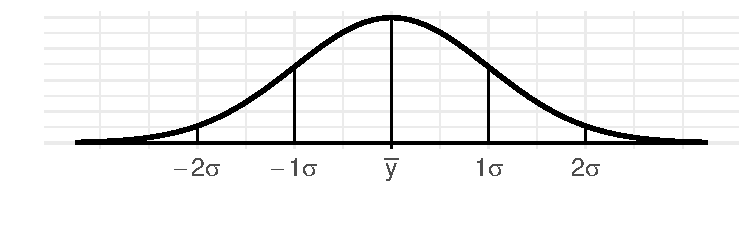
\includegraphics[width=\maxwidth]{img/mc-distribution-02-a-1} 

}







\begin{enumerate}
\item [\textbf{A} \msquare] Dargestellt ist keine Standardnormalverteilung.
\item [\textbf{B} \msquare] Die Fläche unter der Kurve ist 1, wenn die Nullhypothese falsch ist. Wenn die Nullhypothese gilt, dann ist die Fläche $1-\alpha$. Somit ergibt sich auch eine Standardabweichung $\sigma$ mit $\alpha$ gleich 0.05 in beiden Fällen.
\item [\textbf{C} \msquare] Die Fläche links von $-2\sigma$ ist der p-Wert mit $Pr(D|H_0)$ in der obigen Abbildung.
\item [\textbf{D} \msquare] Es liegen 95\% der Beobachtungen zwischen $\bar{y}\pm 2 \sigma$. Angezeigt durch die Fläche zwischen $-2\sigma$ und $2\sigma$ in der obigen Verteilung.
\item [\textbf{E} \msquare] Die Fläche unter der Kurve entspricht dem Signifikanzniveau $\alpha$ von 5\%. Damit ist die Standardabweichung $\sigma$ gleich 1 in der obigen Abbildung.
\end{enumerate} 

\section{Aufgabe \hfill (2 Punkte)}

%% --------------------------------------------------------------------
\ifcollection
\begin{flushright}
\tiny\vspace{-2Ex}
\textbf{\examinhaltstart}
\exammodulemathstat $\;\bullet$
\exammodulestat $\;\bullet$
\exammodulestatbbv $\;\bullet$
\exammodulestatversuch $\;\bullet$
\exammodulebiostat
\vspace{-1Ex}
\end{flushright}
\fi
%% --------------------------------------------------------------------




Die ANOVA ist ein statistisches Verfahren welches häufig in den Auswertungen von Experimenten in den Agrarwissenschaften angewendet
wird. Dabei wird die ANOVA als ein erstes statistischen Werkzeug für die
Übersicht über die Daten benutzt. Eine ANOVA testet dabei...



\begin{enumerate}
\item [\textbf{A} \msquare] ... den Unterschied zwischen der Varianz ausgelöst durch alle Behandlungsgruppen und der Varianz aus globalen Behandlungsguppen der Kontrollen. Wenn die ANOVA nicht signifikant ist, muss ein Posthoc-Test ausgeschlossen werden.
\item [\textbf{B} \msquare] ... den Unterschied zwischen der Mittelwerte und der Varianz aus verschiedenen Behandlungsguppen. Wenn die ANOVA signifikant ist, ist bekannt welcher Vergleich konkret unterschiedlich ist.
\item [\textbf{C} \msquare] ... den Unterschied zwischen der Varianz über alle Behandlungsgruppen oder der Varianz aus verschiedenen Behandlungsguppen. Wenn die ANOVA signifikant ist, muss sich zwischen einem der beiden Varianzquellen entschieden werden.
\item [\textbf{D} \msquare] ... den Unterschied zwischen der F-Statistik anhand der Varianz der Gruppen. Wenn die F-Statistik exakt 0 ist, kann die Nullhypothese abgelehnt werden.
\item [\textbf{E} \msquare] ... den Unterschied zwischen der Varianz über alle Behandlungsgruppen und der Varianz aus verschiedenen Behandlungsguppen. Wenn die ANOVA signifikant ist, muss ein Posthoc-Test angeschlossen werden.
\end{enumerate}

\section{Aufgabe \hfill (2 Punkte)}

%% --------------------------------------------------------------------
\ifcollection
\begin{flushright}
\tiny\vspace{-2Ex}
\textbf{\examinhaltstart}
\exammodulemathstat $\;\bullet$
\exammodulestat $\;\bullet$
\exammodulestatbbv $\;\bullet$
\exammodulestatversuch $\;\bullet$
\exammodulebiostat
\vspace{-1Ex}
\end{flushright}
\fi
%% --------------------------------------------------------------------




Die Ergebnisse der einer statistischen Analyse können in die Analogie einer Wettervorhersage gebracht werden. Welche Analogie für die Ergebnisse eines statistischen Tests trifft am besten zu?



\begin{enumerate}
\item [\textbf{A} \msquare] In der Analogie der Maximaltemperatur: Was ist der maximale Unterschied zwischen zwei Gruppen. Wir erhalten hier eine Aussage über die Spannweite und den maximalen Effekt.
\item [\textbf{B} \msquare] In der Analogie des Niederschlags oder Regenmenge: ein statistischer Test gibt die Stärke eines Effektes wieder. Zum Beispiel, wie hoch ist der Mittelwertsunterschied.
\item [\textbf{C} \msquare] In der Analogie der Regenwahrscheinlichkeit in einem bestimmten Gebiet: ein statistischer Test gibt die Wahrscheinlichkeit für ein Ereignis in einem Experiment mit den Daten $D$ wieder und lässt sich kaum verallgemeinern.
\item [\textbf{D} \msquare] In der Analogie der Regenwahrscheinlichkeit: ein statistischer Test gibt die Wahrscheinlichkeit für das Auftreten eines Ereignisses wieder. Die Stärke des Effektes wird nicht wiedergeben.
\item [\textbf{E} \msquare] In der Analogie der Durchschnittstemperatur: Wie oft tritt ein Effekt durchschnittlich ein? Wir erhalten eine Wahrscheinlichkeit für die Effekte. Zum Beispiel, wie hoch ist die Wahrscheinlichkeit für einen Mittelwert als Durchschnitt.
\end{enumerate} 

\section{Aufgabe \hfill (2 Punkte)}

%% --------------------------------------------------------------------
\ifcollection
\begin{flushright}
\tiny\vspace{-2Ex}
\textbf{\examinhaltstart}
\exammodulestatversuch $\;\bullet$
\exammodulebiostat
\vspace{-1Ex}
\end{flushright}
\fi
%% --------------------------------------------------------------------




Neben der klassischen Regression kann die Funktion \texttt{lm()} in \Rlogo auch für welche andere Art von Anwendung genutzt werden?





\begin{enumerate}
\item [\textbf{A} \msquare] Ist die Einflussvariable $X$ ein Faktor so werden die Gruppenmittelwerte geschätzt und eine anschließende ANOVA sowie multipler Gruppenvergleich mit \{emmeans\} ist möglich. Die Funktion \texttt{lm()} kann dabei eigentlich weggelassen werden, wird aber traditionell gerechnet.
\item [\textbf{B} \msquare] Neben der klassichen Verwendung der Funktion \texttt{lm()} in der linearen Regression kann auch ein Gruppenvergleich gerechnet werden. Dafür müssen aber alle Faktoren aus den Daten entfernt und numerishc umgewandelt werden. Dann kann das R Paket \{emmeans\} genutzt werden um die Korrelation zu berechnen. Eine Adjustierung ist dann nicht mehr notwendig.
\item [\textbf{C} \msquare] Die Funktion \texttt{lm()} in \Rlogo ist der erste Schritt für einen Gruppenvergleich. Danach kann eine ANOVA oder aber ein multipler Vergleich in \{emmeans\} gerechnet werden. In der Funktion  \texttt{lm()} werden die Gruppenmittelwerte bestimmt.
\item [\textbf{D} \msquare] Die Funktion \texttt{lm()} berechnet die Varianzstruktur für eine ANOVA. Dannach kann dann über eine explorative Datenalayse nochmal eine Signifikanz berechnet werden. Sollte vor der Verwendung der Funktion \texttt{lm()} schon eine EDA gerechnet worden sein, so ist die Analyse wertlos.
\item [\textbf{E} \msquare] Die Funktion \texttt{lm()} in \Rlogo ist der letzte Schritt für einen Gruppenvergleich. Vorher kann eine ANOVA oder aber ein multipler Vergleich in \{emmeans\} gerechnet werden. In der Funktion  \texttt{lm()} werden die Gruppenvarianzen bestimmt.
\end{enumerate}

% -----------------------------------------------------------------------
\clearpage
% -----------------------------------------------------------------------

\section{Aufgabe \hfill (12 Punkte)}

\textit{Geben Sie grundsätzlich Formeln und Rechenweg zur Lösung der Teilaufgaben mit an!} \\[1Ex]
 

 
%% --------------------------------------------------------------------
\ifcollection
\begin{flushright}
\tiny\vspace{-3Ex}
\textbf{\examinhaltstart}
\exammodulestatversuch $\;\bullet$
\exammodulebiostat
\vspace{-4Ex}
\end{flushright}
\begin{minipage}[t]{0.5\textwidth}

\includegraphics[width = 1.3cm]{C:/Users/jokruppa/Documents/GitHub/exam/avatare/Mark.png}
\end{minipage}
\begin{minipage}[t]{0.5\textwidth}
\hfill
\href{https://youtu.be/rWTyHXXlYjY}{
\includegraphics[width = 2cm]{img/youtube}}
\end{minipage}
\vspace{-3Ex}
\fi
%% --------------------------------------------------------------------



\ifcollection
\paragraph{Die zweifaktorielle ANOVA in \Rlogo}
\fi

Es ist schon kurz nach fünf und Mark wird langsam nervös. Mark wollte heute Abend noch seine E-Sport Qualifikation schauen. Stattdessen versucht sein Betreuer die Ausgabe der zweifaktoriellen ANOVA zu visualieren und zu überprüfen, ob es mit der Visualisierung der Daten als Boxplots zusammenpasst. Mark hatte im Wendland ein Feldexperiment mit Maiss durchgeführt. Es gab dabei zwei Behandlungen. Einmal Substrattypen ($torf$, $40p60n$, $30p20n$ und $70p30n$) sowie als zweite Behandlung Genotypen ($AA$, und $BB$). Gemessen wurde der Messwert ($Y$) Frischegewicht [kg/ha]. So kompliziert kann das jetzt doch nicht sein! Eigentlich wollte Mark nachher noch zum Sport. Um zu Reiten geht Mark dann später nochmal raus. Echte Entspannung.

\begin{knitrout}
\definecolor{shadecolor}{rgb}{0.969, 0.969, 0.969}\color{fgcolor}\begin{kframe}
\begin{verbatim}
## Analysis of Variance Table
## 
## Response: Frischegewicht
##                         Df Sum Sq Mean Sq F value Pr(>F)
## Substrattypen            2 102.94  51.469  2.0976 0.1518
## Genotypen                1  42.01  42.012  1.7121 0.2072
## Substrattypen:Genotypen  2 254.75 127.377  5.1911 0.0166
## Residuals               18 441.68  24.538
\end{verbatim}
\end{kframe}
\end{knitrout}

\vspace{1ex}

Leider kennt sich Mark mit Berechnung einer zweifaktoriellen ANOVA überhaupt nicht aus. Deshalb braucht er bei der Erstellung Ihre Hilfe! 

\begin{enumerate}
  \item Formulieren Sie die wissenschaftliche Fragestellung für beide Faktoren separat! \textbf{(2 Punkte)}
  \item Formulieren Sie die statistischen Hypothesenpaare für beide Faktoren separat! \textbf{(2 Punkte)}
\item Interpretieren Sie das Ergebnis der zweifaktoriellen ANOVA! Begründen Sie Ihre Antwort! \textbf{(3 Punkte)} 
\item Zeichnen Sie eine Abbildung, der dem obigen Ergebnis der
  zweifaktoriellen ANOVA näherungsweise entspricht! \textbf{(5 Punkte)}
\end{enumerate}
 
\clearpage
% -----------------------------------------------------------------------

\section{Aufgabe \hfill (9 Punkte)}

\textit{Geben Sie grundsätzlich Formeln und Rechenweg zur Lösung der Teilaufgaben mit an!} \\[1Ex]
 

 
%% --------------------------------------------------------------------
\ifcollection
\begin{flushright}
\tiny\vspace{-3Ex}
\textbf{\examinhaltstart}
\exammodulemathstat $\;\bullet$
\exammodulestat $\;\bullet$
\exammodulestatbbv $\;\bullet$
\exammodulestatversuch\\
\exammodulelanddaten $\;\bullet$
\exammodulebiostat
\vspace{-4Ex}
\end{flushright}
\begin{minipage}[t]{0.5\textwidth}

\includegraphics[width = 1.3cm]{C:/Users/jokruppa/Documents/GitHub/exam/avatare/Mark.png}
\end{minipage}
\begin{minipage}[t]{0.5\textwidth}
\hfill
\href{https://youtu.be/Xf0yE-o7bEU}{
\includegraphics[width = 2cm]{img/youtube}}
\end{minipage}
\vspace{-3ex}
\fi
%% --------------------------------------------------------------------



\ifcollection
\paragraph{Zerforschen des Boxplots}
\fi

Boxplots sind bedeutend in der Darstellung von wissenschaftlichen Ergebnissen. Leider hat sich Mark nicht gemerkt, welche statistischen Maßzahlen für einen Boxplot erhoben werden müssen. Besser wäre was anderes gewesen. Am Ende dann doch besser Geocaching. Wunderbar. Eine echte Ablenkung für Mark. Das ist in soweit doof, da nach seiner Betreuerin erstmal ein Boxplot nachgebaut werden soll, bevor es mit seiner Hausarbeit losgeht. Dann hat er schonmal den \Rlogo Code vorliegen und nachher geht dann alles schneller. Na dann mal los. Mark schafft sich die nötige Stimmung. Wenn Andrea Berg ertönt, dann sucht der Hamster schleunigst Schutz unter dem Sofa. Mark schüttelt den Kopf. In der Behandlung für Erbsen werden verschiedene Genotypen ($AA$, $AB$ und $BB$) sein. Erfasst wird als Messwert ($Y$) \textit{Ertrag}. Mark soll dann \textit{yield} in seiner Exceldatei eintragen. Aber nur in passender Atmospäre! Hm, lecker Marzipankugeln und dazu dann im Hintergrund Columbo laufen lassen.



{\centering 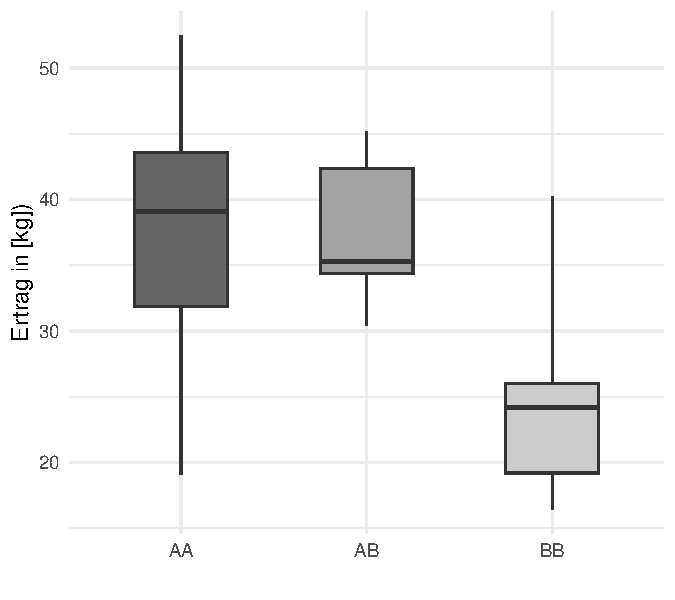
\includegraphics[width=\maxwidth]{img/boxplot-02-zer-1} 

}




Leider kennt sich Mark mit der Erstellung von Boxplots in \Rlogo nicht aus. Deshalb braucht er bei der Visualisierung Ihre Hilfe!

\begin{enumerate}
\item Erstellen Sie eine Tabelle mit den statistischen Maßzahlen aus der obigen Abbildung der drei Boxplots! \textit{Beachten Sie die korrekte Darstellungsform der statistischen Maßzahlen!} \textbf{(3 Punkte)}
\item Beschriften Sie \textit{einen} der Boxplots mit den gängigen statistischen Maßzahlen! \textbf{(2 Punkte)}
\item Erstellen Sie einen beispielhaften Datensatz, aus dem die drei Boxplots \textit{möglicherweise} erstellt wurden, im \Rlogo üblichen Format! \textbf{(2 Punkte)}
\item Kann Mark einen Unterschied zwischen den Behandlungen erwarten? Begründen Sie Ihre Antwort! \textbf{(2 Punkte)}
\end{enumerate} 
\clearpage
% -----------------------------------------------------------------------

\section{Aufgabe \hfill (12 Punkte)}

\textit{Geben Sie grundsätzlich Formeln und Rechenweg zur Lösung der Teilaufgaben mit an!} \\[1Ex]
 

 
%% --------------------------------------------------------------------
\ifcollection
\begin{flushright}
\tiny\vspace{-3Ex}
\textbf{\examinhaltstart}
\exammodulestat $\;\bullet$
\exammodulestatbbv $\;\bullet$
\exammodulestatversuch 
\vspace{-4Ex}
\end{flushright}
\begin{minipage}[t]{0.5\textwidth}

\includegraphics[width = 1.3cm]{C:/Users/jokruppa/Documents/GitHub/exam/avatare/Jessica.png}\hspace{-4mm}
\includegraphics[width = 1.3cm]{C:/Users/jokruppa/Documents/GitHub/exam/avatare/Mark.png}
\end{minipage}
\begin{minipage}[t]{0.5\textwidth}
\hfill
\href{https://youtu.be/lJp8rFmMnrs}{
\includegraphics[width = 2cm]{img/youtube}}
\end{minipage}
\fi
%% --------------------------------------------------------------------



\ifcollection
\paragraph{Interpretation der Ergebnisse einer linearen Regression}
\fi

'Wichtig ist es, dass wir jetzt eine Gerade durch die Punkte zeichnen!', ruft Jessica. 'Ich sehe nur zwei Zeilen und keine Punkte. Wie soll ich da denn jetzt eine Gerade durchzeichnen?', fragt Mark. Jessica atmet schwer ein und starrt auf die \Rlogo Ausgabe der Funktion \texttt{lm()}. Die beiden hatten einen Leistungssteigerungsversuch im Wendland mit Schweinen durchgeführt. Dabei wurden die beiden folgenden Variablen gemessen: mittlere Anzahl an weißen Blutkörperchen [LEU/ml] und Gewichtszuwachs in der 1LW. Das Bestimmtheitsmaß $R^2$ hatten die beiden mit 0.3 bestimmt.  Jetzt will die Betreuung von den beiden einmal die Visualisierung der Daten und auch gleich noch die lineare Regression gerechnet bekommen. Das haben beide in \Rlogo gemacht, aber wie soll das jetzt gehen?

\begin{table}[!h]
\centering\begingroup\fontsize{11}{13}\selectfont

\begin{tabular}{ccccc}
\toprule
term & estimate & std.error & t statistic & p-value\\
\midrule
(Intercept) & 2.31 & 2.21 &  & \\
Mittlere Anzahl & 1.95 & 0.22 &  & \\
\bottomrule
\end{tabular}
\endgroup{}
\end{table}



Leider kennen sich Jessica und Mark mit der linearen Regression für kontinuierliche Daten in \Rlogo überhaupt nicht aus. Deshalb brauchen beide bei der Erstellung Ihre Hilfe!

\begin{enumerate}
\item Formulieren Sie die wissenschaftliche Fragestellung! \textbf{(1 Punkt)}
\item Formulieren Sie die Regressionsgleichung! \textbf{(1 Punkt)}
\item Erstellen  Sie  eine  Visualisierung  der \texttt{lm()}-Ausgabe. \textit{Beachten Sie die Informationen zum Bestimmtheitsmaß $R^2$ aus dem Aufgabentext!} Beschriften  Sie  die  Achsen! \textbf{(2 Punkte)}
\item Beschriften Sie die Visualisierung mit den statistischen Maßzahlen der der \texttt{lm()}-Ausgabe! \textbf{(2 Punkte)}
\item Ergänzen Sie die t-Statistik in der \texttt{lm()}-Ausgabe! \textbf{(2 Punkte)}
\item Ergänzen Sie den $p$-Wert in der \texttt{lm()}-Ausgabe mit $T_{\alpha = 5\%} = 1.96$!  \textbf{(2 Punkte)}
\item Interpretieren Sie den $p$-Wert im Kontext der wissenschaftlichen Fragestellung! \textbf{(1 Punkt)}  
\item Wie groß ist der Effekt im Kontext der wissenschaftlichen Fragestellung? \textbf{(1 Punkt)}
\end{enumerate} 
\clearpage
% -----------------------------------------------------------------------

\section{Aufgabe \hfill (10 Punkte)}


 
%% --------------------------------------------------------------------
\ifcollection
\begin{flushright}
\tiny
\textbf{\examinhaltstart}
\exammodulestatversuch $\;\bullet$
\exammodulebiostat
\vspace{-4Ex}
\end{flushright}
\begin{minipage}[t]{0.5\textwidth}

\includegraphics[width = 1.3cm]{C:/Users/jokruppa/Documents/GitHub/exam/avatare/Jonas.png}\hspace{-4mm}
\includegraphics[width = 1.3cm]{C:/Users/jokruppa/Documents/GitHub/exam/avatare/Paula.png}
\end{minipage}
\begin{minipage}[t]{0.5\textwidth}
\hfill
\href{https://youtu.be/CN_O4fYPbhs}{
\includegraphics[width = 2cm]{img/youtube}}
\end{minipage}
\fi
%% --------------------------------------------------------------------



\ifcollection
\paragraph{Visualisierung des 95\% Konfidenzintervalls}
\fi

'Okay, für was war jetzt nochmal das 95\% Konfidenzintervall gut?', fragt Paula und schaut in das leere Gesicht von Jonas. 'Keine Ahnung. Irgendwas mit Relevanz und Effekt oder Signifikanz. Da kannst du irgendwie was verbinden. Keine Ahnung warum', entgegnet Jonas. 'Wir haben doch als Messwert \textit{Energieverbrauch der Klimakammer} erhoben.', stellt Paula fest. Jetzt haben beide das Problem, die möglichen 95\% Konfidenzintervalle zu interpretieren.

\vspace{1ex}

Leider kennen sich Paula und Jonas mit der Visualisierung des 95\% Konfidenzintervall überhaupt nicht aus. 

\begin{enumerate}
\item Beschriften Sie die untenstehende Abbildung mit der Signifikanzschwelle! Begründen Sie Ihre Antwort! \textbf{(2 Punkte)}
\item Ergänzen Sie eine \textit{in den Kontext passende} Relevanzschwelle! Begründen Sie Ihre Antwort! \textbf{(2 Punkte)} 
\item Skizieren Sie in die untenstehende Abbildung sechs einzelne Konfidenzintervalle (a-f) mit den
  jeweiligen Eigenschaften! \textbf{(6 Punkte)}
  \begin{itemize}
  \item[(a)] Ein signifikantes, relevantes 90\% Konfidenzintervall. 	
  \item[(b)] Ein signifikantes, relevantes 95\% Konfidenzintervall 	
  \item[(c)] Ein signifikantes, nicht relevantes 95\% Konfidenzintervall 	
  \item[(d)] Ein 95\% Konfidenzintervall mit h{"o}herer Varianz $s_p$ in der Stichprobe als der Rest der 95\% Konfidenzintervalle 
  \item[(e)] Ein 95\% Konfidenzintervall mit niedriger Varianz $s_p$ in der Stichprobe als der Rest 95\% der Konfidenzintervalle
  \item[(f)] Ein nicht signifikantes, nicht relevantes 95\% Konfidenzintervall
  \end{itemize}
\end{enumerate}

\begin{center}
  
\includegraphics[height = 10cm]{C:/Users/jokruppa/Documents/GitHub/exam/question/img/statistisches-testen-04}
\end{center}


 
\clearpage
% -----------------------------------------------------------------------

\section{Aufgabe \hfill (10 Punkte)}

\textit{Geben Sie grundsätzlich Formeln und Rechenweg zur Lösung der Teilaufgaben mit an!} \\[1Ex]
 

 
%% --------------------------------------------------------------------
\ifcollection
\begin{flushright}
\tiny\vspace{-3Ex}
\textbf{\examinhaltstart}
\exammodulemathstat $\;\bullet$
\exammodulestat $\;\bullet$
\exammodulestatbbv $\;\bullet$
\exammodulestatversuch $\;\bullet$
\exammodulebiostat
\vspace{-4Ex}
\end{flushright}
\begin{minipage}[t]{0.5\textwidth}

\includegraphics[width = 1.3cm]{C:/Users/jokruppa/Documents/GitHub/exam/avatare/Nilufar.png}
\end{minipage}
\begin{minipage}[t]{0.5\textwidth}
\hfill
\href{https://youtu.be/VAqiUdV4WQ0}{
\includegraphics[width = 2cm]{img/youtube}}
\end{minipage}
\vspace{-3ex}
\fi
%% --------------------------------------------------------------------




\ifcollection
\paragraph{Visualisierung des Scatterplots}
\fi

Wenn es nach Nilufar ginge, wäre sie schon längst fertig mit ihrer Hausarbeit. Geht es aber nicht. Nilufar schmeißt noch eine Handvoll Takis Blue Heat in ihren Rachen. Im Hintergrund klirrt leise der Spiegel zum Sound von Deichkind. In ihrer Hausarbeit hatte sie ein Gewächshausexperiment in der Uckermark durchgeführt. Nach der Meinung ihrer Betreuerin sieht das jedoch etwas anders aus. Jetzt soll sie doch noch eine explorative Datenanalyse für den Zusammenhang zwischen durchschnittlichen Anteil an Ton [\%/l] und Frischegewicht [kg/ha] in Kartoffeln durchführen. Wie nervig! Wenn die Erwartung nicht wäre, ja dann wäre wohl vieles möglich für Nilufar! Aber so.. Da zwei kontinuierliche Variablen vorliegen, geht die explorative Datenanalyse leider nicht mit Boxplots oder Barplots. Dann was anderes. Irgendwie komisch, wenn sie Star Trek anmacht, dann ist das Huhn eigentlich sofort vor dem Bildschirm und starrt hinein.

\begin{table}[!h]
\centering
\begin{tabular}{cc}
\toprule
Frischegewicht [kg/ha] & Durchschnittlichen Anteil an Ton [\%/l]\\
\midrule
19.4 & 20.7\\
24.2 & 16.7\\
16.0 & 10.5\\
22.3 & 19.5\\
17.0 & 15.0\\
\addlinespace
19.7 & 17.9\\
21.2 & 15.4\\
17.6 & 16.9\\
19.9 & 20.1\\
17.6 & 18.9\\
\addlinespace
19.2 & 15.8\\
17.2 & 16.0\\
\bottomrule
\end{tabular}
\end{table}



Leider kennt sich Nilufar mit der Erstellung einer explorativen Datenanalyse für kontinuierliche Daten überhaupt nicht aus. Deshalb braucht sie bei der Erstellung Ihre Hilfe!

\begin{enumerate}
\item Erstellen Sie eine Visualisierung für die Datentabelle. Beschriften Sie
  die Achsen entsprechend! \textbf{(4 Punkte)}
\item Schätzen Sie eine Gerade durch die Punkte! \textbf{(1 Punkt)}
\item Beschriften Sie die Gerade mit den gängigen statistischen Maßzahlen! Geben Sie die numerischen Zahlenwerte mit an! \textbf{(3 Punkte)}
\item Wenn \textit{ein} Effekt von $x$ auf $y$ vorhanden wäre, wie würde die Gerade verlaufen und welche Werte würden die statistischen Maßzahlen annehmen? \textbf{(2 Punkt)}
\end{enumerate} 
\clearpage
% -----------------------------------------------------------------------

\section{Aufgabe \hfill (12 Punkte)}

\textit{Geben Sie grundsätzlich Formeln und Rechenweg zur Lösung der Teilaufgaben mit an!} \\[1Ex]
 

 
%% --------------------------------------------------------------------
\ifcollection
\begin{flushright}
\tiny\vspace{-3Ex}
\textbf{\examinhaltstart}
\exammodulestatversuch $\;\bullet$
\exammodulebiostat
\vspace{-4Ex}
\end{flushright}
\begin{minipage}[t]{0.5\textwidth}

\includegraphics[width = 1.3cm]{C:/Users/jokruppa/Documents/GitHub/exam/avatare/Nilufar.png}\hspace{-4mm}
\includegraphics[width = 1.3cm]{C:/Users/jokruppa/Documents/GitHub/exam/avatare/Paula.png}
\end{minipage}
\begin{minipage}[t]{0.5\textwidth}
\hfill
\href{https://youtu.be/49hvImMwVyE}{
\includegraphics[width = 2cm]{img/youtube}}
\end{minipage}
\fi
%% --------------------------------------------------------------------



\ifcollection
\paragraph{Die einfaktoriellen ANOVA und der Student t-Test}
\fi

'Uff... die einfaktorielle ANOVA. Und wie füllen wir jetzt 	extit{genau} die Tabelle der ANOVA aus und schauen, ob da was signifikant ist?', Paula hebt die Augenbraue. 'Das ist eine sehr gute Frage. Ich glaube man kann alles in der Tabelle relativ einfach mit wenigen Informationen berechnen.', meint Nilufar dazu und schmiß sich noch ein paar Takis Blue Heat in den Rachen. Paula hatte sich in ein Stallexperiment verschiedene Schweinen angeschaut. Dabei ging es herauszufinden, ob es einen Zusammenhang zwischen der Behandlung Genotypen ($AA$, $AB$ und $BB$) und dem Messwert Schlachtgewicht [kg] gibt. Nun möchte erstmal ihre Betreuerin eine ANOVA Tabelle sehen. Was immer da auch drin zu erkennen sein mag. Später wollen die beiden dann noch raus um zu Kicken.



\vspace{1ex}

Leider kennen sich Paula und Nilufar mit Berechnung einer einfaktoriellen ANOVA überhaupt nicht aus. Deshalb brauchen beide bei der Erstellung Ihre Hilfe! 

\begin{enumerate}
  \item Formulieren Sie die wissenschaftliche Fragestellung! \textbf{(1 Punkt)}
  \item Formulieren Sie das statistische Hypothesenpaar! \textbf{(1 Punkt)}
\item Füllen Sie die unterstehende einfaktorielle ANOVA Ergebnistabelle aus! \textbf{(3 Punkte)}
\end{enumerate}

\vspace{1Ex}

\begin{center}
  \Large
  \begin{tabular}{lccccp{3cm}}
\toprule
     & \textbf{Df} & \textbf{Sum Sq} & \textbf{Mean Sq} & \textbf{F value} & \textbf{Pr(>F)} \strut\\
    \midrule
   \textbf{Genotypen}  & 2 & 3068.16 &  &  &  \strut\\
   \textbf{Error}  & 16 & 717.63 &  &  &  \strut\\
\bottomrule
  \end{tabular}
\end{center}

\vspace{1Ex}

\begin{enumerate}
  \setcounter{enumi}{3}
\item Schätzen Sie den p-Wert der Tabelle mit $F_{\alpha = 5\%} = 3.63$ ab. Begründen Sie Ihre Antwort! \textbf{(2 Punkte)}
\item Was bedeutet ein signifikantes Ergebnis in einer einfaktoriellen ANOVA? \textbf{(1 Punkt)}
\item Berechnen Sie \textit{einen} Student t-Test für den \textit{vermutlich} signifikantesten Gruppenvergleich anhand der untenstehenden Tabelle mit $T_{\alpha = 5\%} = 2.03$. Begründen Sie Ihre Auswahl! \textbf{(3 Punkte)}
\end{enumerate}


\begin{knitrout}
\definecolor{shadecolor}{rgb}{0.969, 0.969, 0.969}\color{fgcolor}\begin{table}[!h]
\centering\begingroup\fontsize{11}{13}\selectfont

\begin{tabular}{cccc}
\toprule
\textbf{Genotypen} & \textbf{Fallzahl (n)} & \textbf{Mittelwert} & \textbf{Standardabweichung}\\
\midrule
AA & 8 & 32.00 & 7.23\\
AB & 6 & 5.83 & 1.72\\
BB & 5 & 6.80 & 9.18\\
\bottomrule
\end{tabular}
\endgroup{}
\end{table}

\end{knitrout}


\begin{enumerate}
  \setcounter{enumi}{6}
\item Gegebenen der ANOVA Tabelle war das Ergebnis des Student t-Tests zu erwarten? Begründen Sie Ihre Antwort! \textbf{(2 Punkte)}
\end{enumerate}

 
\clearpage
% -----------------------------------------------------------------------

\section{Aufgabe \hfill (10 Punkte)}

\textit{Geben Sie grundsätzlich Formeln und Rechenweg zur Lösung der Teilaufgaben mit an!} \\[1Ex]
 

 
%% --------------------------------------------------------------------
\ifcollection
\begin{flushright}
\tiny\vspace{-3Ex}
\textbf{\examinhaltstart}
\exammodulestat $\;\bullet$
\exammodulestatbbv $\;\bullet$
\exammodulestatversuch $\;\bullet$
\exammodulebiostat
\vspace{-4Ex}
\end{flushright}
\begin{minipage}[t]{0.5\textwidth}

\includegraphics[width = 1.3cm]{C:/Users/jokruppa/Documents/GitHub/exam/avatare/Mark.png}
\end{minipage}
\begin{minipage}[t]{0.5\textwidth}
\hfill
\href{https://youtu.be/xq29O8qDrg0}{
\includegraphics[width = 2cm]{img/youtube}}
\end{minipage}
\vspace{-3ex}
\fi
%% --------------------------------------------------------------------



\ifcollection
\paragraph{Visualisierung des Compact Letter Displays (CLD)}
\fi

Mark hatte in seinem Projektbericht einen Leistungssteigerungsversuch durchgeführt. Soweit so gut. Dabei hat er sich mit Zandern beschäftigt. Angeblich der neueste heiße Kram... aber das ist wiederum was anderes. So richtig mitgenommen hat Mark das Thema dann doch nicht. Hat er sich doch mit Elterlinie ($ctrl$, $Standard$, $SLOW$, und $Xray$) und Fettgehalt [\%/kg] schon eine Menge an Daten angeschaut. Nach seinem Betreuer soll er nun ein CLD bestimmen. Weder weiß er was ein CLD ist, noch war sein erster Gedanke mit Köln und die LGBTQ Community richtig...

\begin{knitrout}
\definecolor{shadecolor}{rgb}{0.969, 0.969, 0.969}\color{fgcolor}\begin{table}[!h]
\centering\begingroup\fontsize{10}{12}\selectfont

\begin{tabular}{cc}
\toprule
\textbf{Behandlung} & \textbf{Compact letter display}\\
\midrule
ctrl & A\\
Standard & B\\
SLOW & BC\\
Xray & C\\
\bottomrule
\end{tabular}
\endgroup{}
\end{table}

\end{knitrout}

Leider kennen sich Mark mit dem \textit{Compact letter display (CLD)} überhaupt nicht aus. Deshalb braucht er bei der Erstellung Ihre Hilfe!

\begin{enumerate}
  \item Formulieren Sie die wissenschaftliche Fragestellung! \textbf{(1 Punkt)}
  \item Formulieren Sie die statistischen Hypothesen! \textbf{(1 Punkt)}
\item Zeichnen Sie die sich anhand des \textit{Compact letter display (CLD)} ergebenden Barplots! \textbf{(2 Punkte)}
\item Ergänzen Sie das \textit{Compact letter display (CLD)} zu den Barplots! \textbf{(1 Punkt)}
\item Erklären Sie \textit{einen} Vorteil und \textit{einen} Nachteil des \textit{Compact letter display (CLD)}! \textbf{(2 Punkte)}
\item Erstellen Sie eine Matrix mit den paarweisen $p$-Werten eines Student t-Tests, die sich näherungsweise aus dem \textit{Compact letter display (CLD)} ergeben würde! Begründen Sie Ihre Antwort! \textbf{(3 Punkte)}
\end{enumerate}

 
\clearpage
% -----------------------------------------------------------------------
\end{document}
% -----------------------------------------------------------------------


  
